\documentclass[10pt,a4paper]{paper}
\usepackage[utf8]{inputenc}
\usepackage[portuguese]{babel}
\usepackage[T1]{fontenc}
\usepackage{amsmath}
\usepackage{amsfonts}
\usepackage{amssymb}
\usepackage{makeidx}
\usepackage{graphicx}
\author{Duarte Ferreira Dias}
\title{Sebenta AC2}
\begin{document}

\maketitle
\newpage
	\section*{I/O}
	
	\subsection*{Periféricos}
	Os periféricos apresentam uma grande variedade de configurações possíveis no que toca à sua operaçãoo.A velocidade de trasnferência de informação é geralmente reduzida em comparação com a do processador e a da memória.
	São os periféricos que se ligam aos módulos de I/O.
	São os periféricos que permitem fazer a conexão entre o computador e o exterior.
	\begin{flushleft}
		Existem três categorias de periféricos:
	\end{flushleft}
	 \begin{itemize}
  		 \item  Legiveis por Pessoas
   			\begin{itemize}
     			\item usados como dispositivos de interface humana
			\end{itemize}     
       	\item  Legiveis pela máquina
       		\begin{itemize}
      			\item Usados para comunicar com outros dispositivos ou equipamentos. 
     		  \end{itemize}
	        \item  Comunicação
	       		\begin{itemize}
	       			\item Usados para comunicar com dispositivos remotos
	       		\end{itemize}
    	   \end{itemize}

	\subsubsection{Interface com os Módulos de I/O}
	Interface aos Módulos de I/O
	\begin{itemize}
		\item Sinais de Controlo:Determinam a tarefa a desempenhar pelo periférico:
		\begin{itemize}
		\item I/P(Read)- envia dado para o módulo de IO;
		\item O/P(Write) -Recebe dado do módulo de IO;
		\end{itemize}
		\item Sinais de Estado: Informam o módulo de IO do estado  actual do periférico;
		\item Data : Conjunto de bits a serem lidos e escritos pelo módulo de IO;
	\end{itemize}
	
	\begin{flushleft}
		Dentro do periférico temos a seguinte estrutura:	
	\end{flushleft}
	\begin{itemize}
		\item Control Logic : Controla a operação do periférico segundo as directivas do módulo de IO;
		\item Buffer. armazena temporariamente os dados transferidos entre o módulo de IO e o exterior;
		\item Transducer:	 Conversão dos signais electricos.
	\end{itemize}
	\subsection*{Módulos IO}
	Devido à incapacidade de fazer comunicação directa entre os periféricos e o processador torna-se imperativo utilizar módulos que tornem essa comunicação possível, os Módulos de IO conhecido també por IO Adapters.
	
	A comunicação entre um processador e um Módulo de IO pode ser resumida a:
	\begin{itemize}
		\item Descodificação dos Comandos:-O módulo IO recebe do processador comandos através do Control Bus;
	 	\item Dados (Data Bus);
		 \item Estado(Status): - BUSY,READY...;
	 	\item Descodificação do Endereço.;
	\end{itemize}

	
	\subsubsection*{Modelo de Programação}
	
	\begin{flushleft}
	Os módulos I/O tê por norma os segunites registos:
	\end{flushleft}
		\begin{itemize}
		\item Registo de Dados(Data Register): registo onde o processador coloca o dado a ser escrito no periérico e por sua vez é também o registo no qual são guardados os dados fornecidos pelo periférico;
		\item Registo de Estado(Status Register):  é neste registo que ser armazenam os bits relativos ao estado atual do periférico;
		\item Registos de Controlo(Control Register): Registo para o qual são escritos, tal com o nome indica, os comandos que ditam qual a operação a efectuar pelo periférico. Existem quatro tipos de comandos que o módulo de IO recebe do processador:
		\begin{itemize}
			\item Control : Indica ao periférico a função a desempenhar.
			\item Teste: usado para testar as condições de estado associadaas ao módulo de IO e ao periféricos a ele ligado;
			\item Input: Ordena ao módulo de IO que obtenha dados do periférico e que os coloque no seu buffer interno;
			\item Output: Ordena ao módulo de IO que leia um dado pro veniente do Data Bus e que o envie para o periférico.
		\end{itemize}
	\end{itemize}

	\subsubsection*{Tipos de Registos IO}
	Existem duas maneiras de organizar os registos de IO uma delas consiste em agrupar esses registos num espaço de endereçamento especifíco e diferente do espaço de endereçamento de memória, o I/O isolado e em oposição os registos de IO mapeados em memória.	
		
	\paragraph*{I/O isolado}
	
	Este tipo de organização de registos IO faz com que sejam necessárias linhas de seleção diferentes para a memória e os dispositivos de IO.Requerem também comandos especiais de IO(instruções In e Out)
	
	\paragraph*{I/O mapeado em memória}
	
	Com este tipo de organização, tanto a memória como os periféricos partilha o mesmo espaço de endereçamento(Address space). As operações de IO apresentam-se como instruções de write e load na memória, tornando assim desnecessários comandos especificos para IO.
	
	\subsection*{Conversão A/D}
		
	A conversão de analógico para digital consiste na modelção de um sinal analógico para que este tome um de dois valores. Este éum dos módulos mais importantes de um microcontrolador pois tudo o que nos rodei no mundo é analógico, e para processarmos esses sinais temos que os converter em sinais digitais para que possam ser processados digitalmente pelo microprocessador.
	
	\subsection*{Tipos de I/O}
	
	\subsubsection*{I/O programado(polling)}
	
	Ao utuilizar esta forma de interface o computador, ao receber um comando de I/O este envia um comando ao módulo de I/O, que por sua vez executa a ação especificada pelo comando e coloca os bits de estado com os valores pretendidos para a operaçãoa efectuar. O processador lé várias vezes o módulo de IO até que a operação seja concluída.
	Se o processador for mais rápido que o periférico este vai ter ciclos de pura inatividade em termos de processamento, chamam-se a estes periodos de "busy waiting".
	
	\subsubsection*{I/O por interrupção}
	
	As interrupções são o resultado de uma operação normal e são despoletadas pelo módulo de I/O. As excepções podem também surgir associadas a erros de memória, inexistência da instrução  e system calls.
	
	Quando é gerada uma interrupção, o processador para a execução das instruções que estava a executar e passa a executar as intruções expecificadas por rotinas de atendimento à interrupção, ou excepção(interrupt/exception handler).
	
	Em oposição ao método de I/O programado a interface por interrupção  permite que o processador execute trabalho útil enquanto o módulo de IO  exectua as instruçõesz que lhe foram atríbuidas, assim que este termina o seu trabalho, gera uma interrupção avisando o processador que está pronto para trocar dados,  que são posteriormente transferidos para a memória.
	
	\subsubsection*{Identificação do dispositivo que gera a interrupção}
	
	Uma maneira de identificar o dispositivo que pede a interrupção é cada dispositivo positivo ter uma linha de lançamento da interrupção própria, outra é a Interrupt Service Routine procura qual foi o módulo que efectuou o pedidod e interrupção. Assim que é identificado este salta  para a rotina deatendimento da interrupção.
	OPode ainda ser feita uma ligação em Daisy Chain.
	
	
	\subsubsection*{Múltiplas fontes de interrupção}
	
	Para gerir as periridades de interrupção forma encontradas duas soluções.
	Uma delas consiste em efectuar o interrupt disable(desabilitar as interrupções) enquanto uma interrupção está a serprocessado. Esta solução não respionde totalmente à necessidade de gerir prioridades sendo impossível assegurar tempos de resposta.	
	
	Defenindo a prioridade que cada excepção tem é possível interromper a rotina de tratamento de uma interrupção se houver outra com maior prioridade para ser tratada.
	
	\subsubsection{Controle de excepções no MIPS}

No MIPS o controlo de interrupções e excepçoes é efectuado pelo coprocessador0 (CPO ) e dentro deste é assegurado pelo System Control Processor

As excepções podem ser causadads tanto por Hardware como pelo software em si. No caso do hardware estas são geradas por um periférico, já no caso do software esttas são designadas por Traps e são originadas por tentativa de execução de instrução indefinida, breakpoints e system calls.

Quando ocorre uma exccepção esta é registada no Cause Register e é feito um salto para a roti8na de tratamento de excepções(Exception handler).Por fim retorna-se ao ponto de execução em que o programa estava antes da interrupção.

	\paragraph{Registos das Excepções}
	
		Os registos de CP0 não fazem parte do banco de registos do processador:
		\begin{itemize}
			\item Startus Register: controla o registo de estado
			\item Cause: regista a causa da excpção
			\item EPC (exception PC)
		\end{itemize}


	\paragraph*{Tratamento das Excepções}
	
	Numa primeira fase o PC é salvaguardado no registo EPC, de seguida é escrita no registo Cause a causa da excepção ou da interrupção,no terceiro passo o processadr passa para o modo kernal e disables ITs.por fim o processador salta para o Exception Handler.
	
	\subsubsection*{DMA}
	
	Ao fazer I/O sob interrupção as taxas de transferência de informação estão limitadas à velocidade com a qual o processador atende os vários periféricos.
	Quando é necessário transferir uma grande quantidade de informação é mais conveniente usar a técnica de Acesso Direto à memória (DMA).
	
	O módulo DMA é capaz de assumir o controlo do sistema substituindo o processador.
	
	\paragraph{Operação do Módulo de DMA}
	
	...
	
	\newpage
	
	\section*{Buses}
	
	Os Buses representam as linhas que interligam o s diferentes componentwes aos quais o processador se encontra ligado.
	Destacam-se dois tipos de ligações:
	\begin{itemize}
		\item Ligações Ponto-a-Ponto:
		\begin{itemize}
			\item Full crossbar ou Matrix Bus:ligação entre dois componentes através de linhas de ligação decdicadas a essa ligação.
		\end{itemize}
		\item Vias de comunicação(linhas) comuns: partilhadas pelos diferentes sistemasd de conmputação
		\begin{itemize}
			\item Shared Bus: Os vários elementos do sistema encontram-se interligados por linhas partilhadas por todos eles, ou seja,qualquer sinal que seja injectado na linha de transmissão pode ser analizado por qualquer um dos compnentes que esteja ligado a esse bus.
		\end{itemize}
	\end{itemize}
	
	Da utilização de buses destaca-se a grande  versatilidade da prática, pois torna-se fácil de adicionar dispositivos novos ao sistema assim como maior compatibilidade dos periifércos com vários sistemas.Destaca-sae também o baixo custo  pois um úncio conjunto de linhas pode ser utilizado em simultaneo para diferentes comunicações.
	
	Porém a utiluização de buses trás algumas desvantagens tais como a criação de estrangulamentos na comunicaçãoc e a limitação da velocidade do busque é limitada não só pelo seu comprimento, assim como o número de dispositivos ligado ao mesmo mas também pela necessidade de suportar dispositivos com latências diferentes e taxas de transferência de dados distintas.\\
	
	\begin{flushleft}
	\textbf{Módulos ligados ao Bus}:	
	\end{flushleft}

	\begin{itemize}
		\item \textbf{Memória}: tem N posições com endereço compreendido entre (0,1...,N-1).Uma palavra pode ser escrita ou lida da memória através dos sinas de controle Read and Write.
		\item \textbf{Modulo I/O}
		\begin{itemize}
			\item \textbf{M Portas}: Cada módulo de IO pode controlar um número (M) de periféricos.Apresenta um endereçamento semelhante à memória.
			\item \textbf{External Data}  linhas de entrada e saída de dados do periférico.
			\item \textbf{Interrupt Signals}
		\end{itemize}
		\item \textbf{Processador}
	\end{itemize}	
			
	\begin{figure}[ht]
		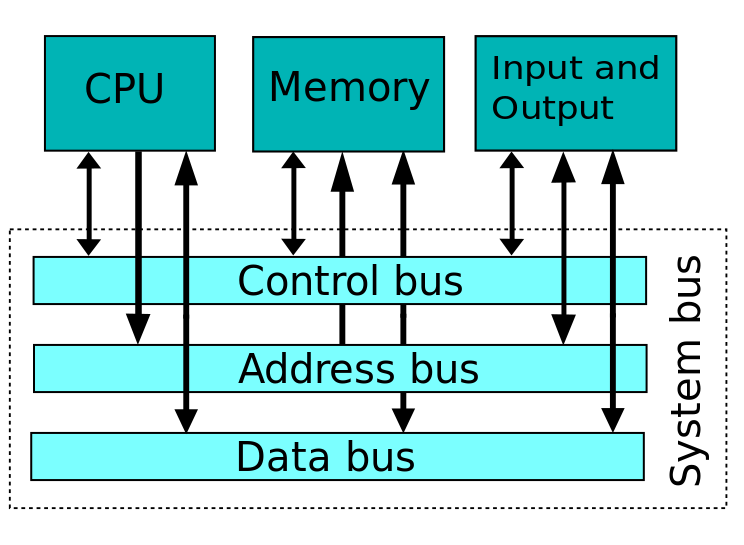
\includegraphics[scale=0.4]{fig1.png}
		\centering
		\caption{Representação gráfica das lligações de um BUS}
		\label{fig:figura 1}
	\end{figure}
	
	
Como se pode ver na figura \ref{fig:figura 1} é possivel distinguir três tipose de bus, o bus de dados, o bus de endereços e o bus de controle.

	\subsection*{Tipos de Buses}
	\subsubsection*{Data Bus}
	As linhas de dados são ligações que permitem a transferênciad de dados entre os blocos de componentes do sistema. Pode ter 32 ou mais linhas, esse numero está diretamente relacionado com a a largura do bus e determina quantos bits podem ser transferidos em simultâneo.
	
	\subsubsection*{Address Bus(Endereçamento)}
	Este bus é utilizado para definir qual a origem e o destino dos dados que circulam num BUS. A largura deste Bus define a  quantidade de memória que o sistema pode levar. è também usado para efectuar endereçamento dos portos de I/O.
	
	\subsubsection*{Control Bus}
	
	Usado para controlar o acesso e o uso das linhas de dados e endereçamento o Control Bus  transmite também sinaios de controlo que definem os comandos e a temporização dos módulos do sistema.
	
	\subsection*{Tipos de Dispositivos ligados ao BUS}
	
	\subsubsection*{Master}
	Os dispositivos do tipo master podem iniciar uma transferência de dados(Read,Write). Exemplos destes dispositivos são o processador e o módulo de I/O, caso seja operado com acesso direto à memória(DMA).

	\subsubsection*{Slave}
	O Slave é um dispositivo que apenas responde a pedidos de trânsferência de Dados.Exemplos são a memória e o módulo de I/O desta vez sem DMA.
	
	\begin{figure}[ht]
		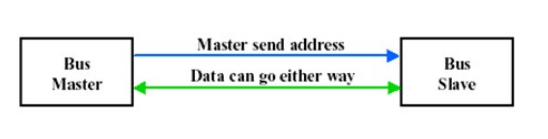
\includegraphics[scale=0.4]{fig2.png}
		\centering
		\caption{Representação gráfica das lligações de um BUS}
		\label{fig:figura2 }
	\end{figure}
	
	Existem vários protocolos usados para comunicar entre dispositivos que partilham o mesmo bus.
	
 \subsection*{Bus Paralelo}
 
 Qua  ndo o bus é paralelo como o nome indica os dados são transferidos em paralelo, tornando, assim mais rápida a transfência de dados. É caro aplicar este tipo de buses em grande distância assim como há existência de interferência entre pistas quando são usadas altas frequências.
 
 \subsection*{Bus Série}
 
A  implementação deste tipo de Bus é muito barata e adequada a transmissão a grandes distâncias, mas é mais lento.

\subsection*{Bus Sincrono}

Caracteristicas :
\begin{itemize}
\item Inclui uma linha de relógio;
\item Protocolo de comunicação fixo, relativo ao relógio;
\item Vantagens: lógica de interface simples e rápida.
\item Desvantagens;
	\begin{itemize}
		\item Todos os dispositivos que estão ligados ao bus são obrigados a trabalhar à mesma frequência;
		\item O comprimento do us depende da frequência de relógio com vista a evitar desvios do relógio;
	\end{itemize}
\end{itemize}

\begin{flushleft}
	Transações no Bus Síncrono:
\end{flushleft}

\begin{enumerate}
	\item CPU coloca enderço da palavra que quer  ler nas linhas de endereço;
	\item Após as tensões da linha de endereçamento estabilizarem O CPU ativa as linhas MREQ(Memory Request) e RD(Read);
	\item Como a memória não pde fornecer dados durante T2, ativa Wait para indicar ao processador o estado de Wait;
	\item A memória colocara no Data Bus a informação em T3 e indica-o desativando o WAIT;
	\item A memória coloca  conteúdo da posição endereçada nas linhas de dados;
	\item Finalmente, o CPU lê e coloca o valor nas linhas de estado e desativa MREQ e RD libertando o bus.
\end{enumerate}

	\begin{figure}[ht]
		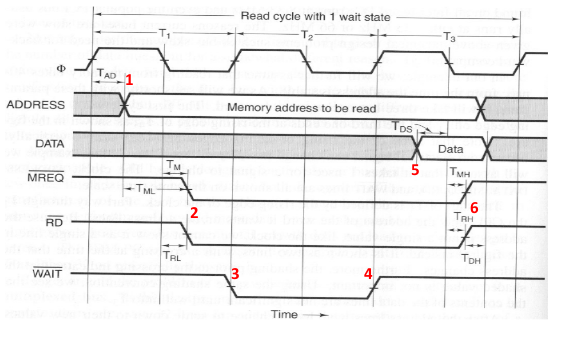
\includegraphics[scale=0.7]{fig3.png}
		\centering
		\caption{Transições de um BUS síncrono}
		\label{fig:figura2 }
	\end{figure}



\subsection*{Bus Assíncrono}

Caracteristicas:
\begin{itemize}
	\item Não há relógio;
	\item Suporta a ligação de uma grande variedade de dispositivos operando a diferentes frequências;
	\item necessário protocolo de \textit{\textbf{handshaking}}, porém este introduz dois tempos de propagação tornando, assim. o bus  mais lento.
\end{itemize}

\begin{flushleft}
	\textbf{Transações no Bus Assíncrono:}
\end{flushleft}

\begin{enumerate}
	\item CPU coloca endereços no BUS;
	\item CPU ativa as linhas MREQ(Memory Request) e RD(Read);
	\item CPU ativa MSYN;
	\item Controldador de Memória coloca o conteúdo da posição endereçadanas linhas de dados e activa SSYN;
	\item O CPU lê os valres nas linhas de dados e desativa MREQ, RD e MSYN;
	\item Finalmente, controlador de memória desativa SSYN.
\end{enumerate}

	\begin{figure}[ht]
		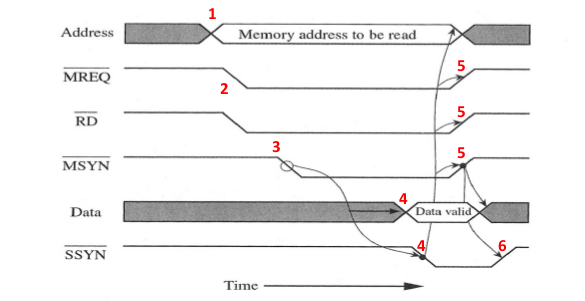
\includegraphics[scale=0.7]{fig4.png}
		\centering
		\caption{Transições de um BUS Assíncrono}
		\label{fig:figura2 }
	\end{figure}



\subsubsection*{Handshake}

Os sinais de hanshake são todos aqueles que têm relação de causa-efeito.

No exemplo anterior dis-ze que o protocolo é \textbf{\textit{full handshake}}.

\subsection*{Arbitragem do  BUS}

Quando á mais que um módulo master pode haver conflitos entre as transferências dos dados. Torna-se imperativo arbitrar o BUS.

\subsubsection*{Arbitragem Centralizada}

Neste tipo de arbitragem a decisão de atribuição do bus é feita por um dispositivo espceifico chamdo árbitro.
A descodificação de endereços é feita por um decoder que tem como input as linhas de endereçamento do bus e gera os bits de seleção do módulo slave respectivo.
O árbitro tem como entradas as linhas de Bus Request dos masters e a sua saída as linhas de Bus Grant.

Ao utilizar este dipo de arbitragem torna-se fácil adicionar novos módulos ao bus, porém é limitado pelo numero de linhas de Bus Reguest e Grant do Master.




\subsubsection*{Arbitragem Distribuida}

	
	\begin{figure}[ht]
		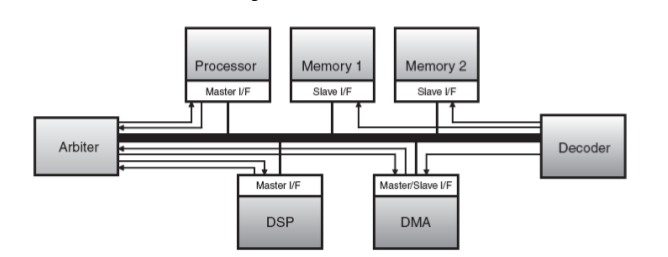
\includegraphics[scale=0.5]{fig5.png}
		\centering
		\caption{Arbitragem Centralizada}
		\label{fig:figura2 }
	\end{figure}
	
	\begin{figure}[ht]
		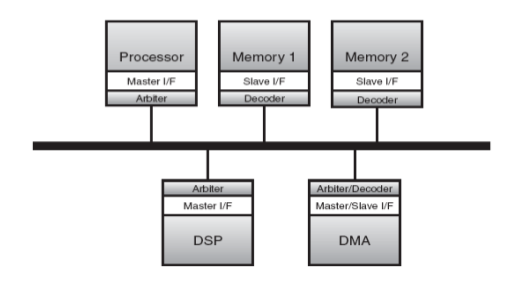
\includegraphics[scale=0.5]{fig6.png}
		\centering
		\caption{Arbitragem Distribuída}
		\label{fig:figura2 }
	\end{figure}
	
	
	\subsubsection*{Politicas de arbitragem:}

\begin{enumerate}
 \item Prioridade Fixa: a cada um do \textit{masters} no bus é atribuída uma prioridade fixa:
 	\begin{itemize}
 		\item Non-pre-emptive :uma vez obtido o	controle do	bus	o	módulo mantem-no	
até terminar a	transferência,	mesmo se	no	decorrer desta um	módulo de	
prioridade mais elevada formule um	bus	request;
		\item Pre-emptive:uma transferência de	prioridade mais baixa é interrompida por
um	pedido de	acesso de	um	módulo com	prioridade mais elevada;
		\item Consequência-> Starvation:módulos de	prioridade mais baixa não conseguem aceder
ao bus	em tempo	util;
 	\end{itemize}
	\item Round-Robin: acesso ao bus	é atribuído rotativamente – um	master
quando termina a	transferência passa o	controle ao master seguinte

	\item Prioridade dinâmica:-prioridades podem variar em runtime	 (com	o	
sistema ligado)	consoante o	perfil de	tráfico das	aplicações
\end{enumerate}	
		

	
	\subsection*{PCI}
		Dos vários buses existentes na indústria destacam-se o Unibus, o Multibus, o USB, o ISA e EISA bus, o PCI, PCIe,Camac,Firewire e o VMEbus.
		
	Também conhecido por Peripheral Component Interconnect o PCI foi um dos buses mais usados na industria dos computadores pessoais para poder ligar todos os periféricos do computador ao processador, tendo evoluido para o PCI Express.
	
	O PCI é um bus síncrono com um relógio de 33MHz ou 66 MHz, é multiplexado, ou seja, tem linhas comuns(32 ou 64 Address/Data lines) para os endereços e os dados. Existe em versões de 32 e 64bit e tem arbitragen centralizada.
	 
	
	\subsubsection*{Estrutura do Bus}
	
	\begin{itemize}
		\item System Pins -linhas de clock e reset;
		\item Address e Data pins:
		\begin{itemize}
			\item AD[31::0] - linhas multiplexadas para endereços e dados;
			\item C/BE[3::0] - linhasmultiplexadas comando/byte enable.
		\end{itemize}
		\item Interface Control Pins
		\begin{itemize}
			\item FRAME\# indica o inicio e duração da transação;
			\item IRDY\# Initittor Ready;
			\item TRDY\#:Target Ready;
			\item DEVSEL\#: Device Select:ativado pelo target quando reconheceu o seu endereço.Indica ao master atual que foi selecionado um dispositivo.
		\end{itemize}
	\end{itemize}
	
	
	\subsection*{PCIe}
	
	Em oposição ao PCI  o PCIe usa ligação ponto a ponto ao invés de um bus partilhado, opta também pela a utilização de Buses em série.Tem a comunicação encapsulada ao invés de enviar os bits directamente.(a aprofundar)
	
	
	\section*{Comunicação}
	
	Existem duas alternativas para a comunicação de um computador com o exterior.A comunicação em série e a comunicação em paralelo.
	
	\subsection*{Comunicação em Série}
		
		Este é o tipo de comunicação preferida pelo mercado havendo vários protocolos diferentes para este tipo de transmissão tais como o USB, o SPI , R-232C e I2C.
		A comunicação é mais lenta pois é feita bit a bit.
	
	\subsection*{Comunicação em Paralelo}
	
	Com este tipo de comunicação é possível enviar vários bits em simultãneo, porém só pode ser usado em distâncias curtas.è exemplo deste tipo de comunicação o PMP presente no Pic32
	
	\subsection*{Assincrona}
	
	Na transmissão Assíncrona  é necessário adicionar bits que sinalizem o inicio e o fim de um caracter	que neste caso são designados por Start Bit e Stop Bit respectivamente
	
	\begin{figure}[ht]
		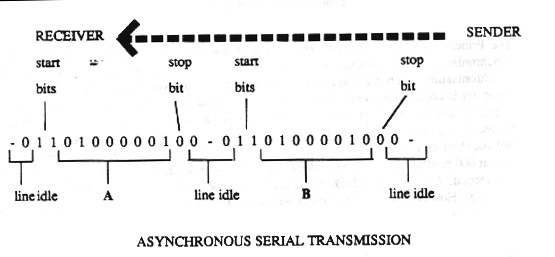
\includegraphics[scale=0.5]{fig7.png}
		\centering
		\caption{Sequênia de transmissão de mensagem em série em modo Assincrono}
		\label{fig:figura7 }
	\end{figure}
	

	\subsection*{Sincrona}
	
Este regime de transmissão implica que os relógios do recetor e transmissor estejam sincronizados.Quando não há transmissão do sinal de relógio é necessário inferir o mesmo a partir das transições de linha.
	
	\subsection*{Códigos de Transmissão} 
	
	Destacam-se quatro códigos de Transmissão(line codes):
	
	\begin{enumerate}
		\item Non-Return to Zero level(NRZL) ;
		\item Non-Return to Zero Inverted(NRZLI): sinal tem uma transição no relógio quando o zero é transmitido e não se altera enquanto houverem 1's a serem transmitidos;
		\item Return to Zero (RZ):sinal volta a zero sempre que há uma transição descendente do flanco do relógio;
		\item Manchester Code: sentido da codificação altera-se a meio do período que codifica o valor, defenindo assim o seu valor lógico.
	\end{enumerate}
	
	\subsubsection*{Código 8b/10b}
	Cada byte de dados(8 bits) é transmitido em palavras de 10bits por forma a facilitar a sua recuperação no receptor. Assim, os valores são divididos em duas palavras cada uma com cinco bits uma delas contém os MSB's e as outras os LSB's 
	 
	
 \subsection*{ Comunicação Série Assincrona: RS-232C}
 
 Este tipo de comunuicação foi utilizada nas primeiras gerações de computadores pessoais com o intuito de entreligar computadores.
 O standard para a transimissão série de dados define  os sinais que ligam um DTE a um DCE.
 Já o Standard para a comunicação RS-232C define as caracteristicas elétricas  dos sinais(high level, low level ....)
 assim como as caracteristicas mecânicas da interface fisica assim como as suas aplicações especifícas.
 
 Os niveis de tensão costumam estar compreendidos acima de ]-3V.3V[ com um máximo de 12V para cada extremo.
 \newpage
 
 \subsubsection*{Exemplo de uma Transmissão ASCII de 8bits sem paridade e NRZ}
 
 	\begin{figure}[ht]
		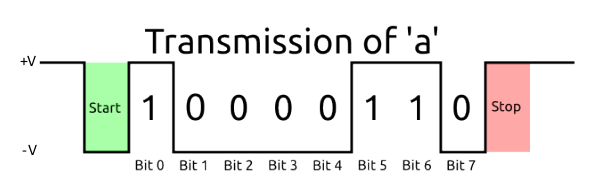
\includegraphics[scale=0.5]{fig8.png}
		\centering
		\caption{Série de bits transmitidos em ASCII usando o protocolo RS-232C}
		\label{fig:figura8 }
	\end{figure}
	
	Na figura \ref{fig:figura8 }  é possível observar a forma como são enviados os dados.
	
	Quanto ao receptor:
	\begin{enumerate}
		\item Detecta bit com transição 1 -> 0 na linha de transmissão;
		\item Usando um relógio, o receptor examina a linha nos nmomentos determinados pela baudrate para determinar os valores dos bits.
	\end{enumerate}
	
 \subsection{Comunicação Série Assincrona: UART}
	
	A UART é  também conhecida por Universal Asynchronous Receiver-Transmitter. 
	Cada UART é munida de um shift register para efectuar a conversão paralelo-série aquando a transmissão e série-paralelo na recepção.
	Esta não costuma enviar sinais directamente para o exterior, sendo este processo assegurado pelo RS-232.
	
\subsubsection*{Transmissão}

A transmissão é feita através do envio de bytes de dados separados por bits individuais.Enumerando:

\begin{enumerate}
	\item O Dado à Cabeça da DIDO é carregado em UxTSR;
	\item A UART gera um Start Bit e através da Serial-Out o bit seguinte do dado a transmitir é colocado à saida a cada ciclo de relógio. O Sentido de transmissão realiza-se no sentido do LSB -> MSB;
	\item A UART gera e transmite bit de paridade e stopbits se assim for especificado.
\end{enumerate}


\subsubsection*{Recepção}
	A recepção limita-se a receber e a voltar a juntar os bits em bytes e processa-se pela seguinte ordem:
	\begin{enumerate}
	\item O Start bit é detectado;
	\item Após o tempo de transmissão de um bit a linha de entrada é novamente amostrada e o valor é processado pelo shift Register;
	\item Depois do tempo de amostragem dos bits da palavra ter decorrido o conteudo do shift regster fica disponivel no buffer do receptor para ser lido em paralelo.A UART ativa uma flag pra indicar que um novo dado está disponivel .
\end{enumerate}



 	\begin{figure}[ht]
		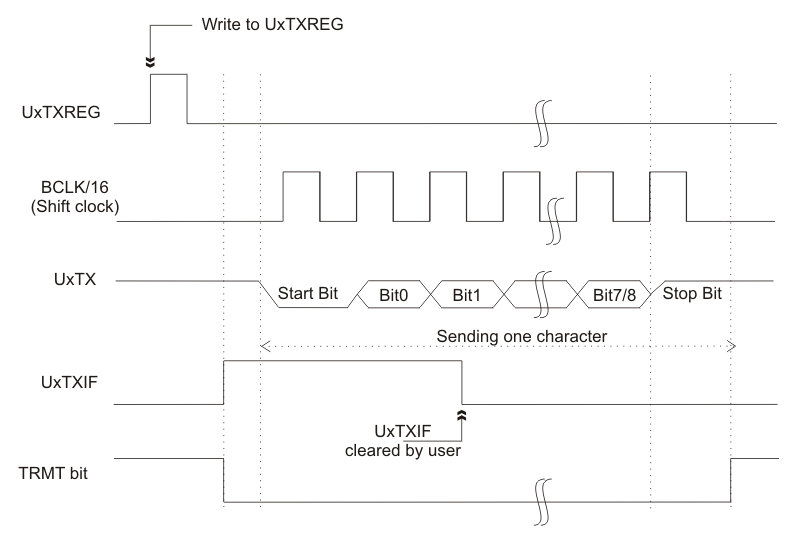
\includegraphics[scale=0.35]{fig9.png}
		\centering
		\caption{Transmissão de bits na UART}
		\label{fig:figura9 }
	\end{figure}
	
 	\begin{figure}[ht]
		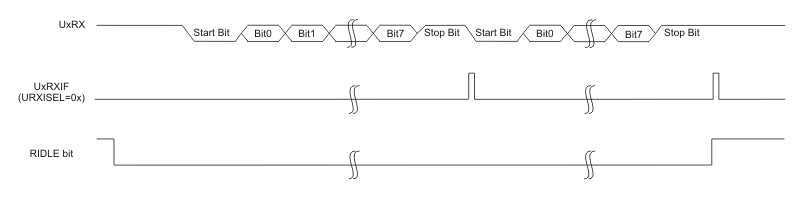
\includegraphics[scale=0.35]{fig10.png}
		\centering
		\caption{Recepção de bits na UART}
		\label{fig:figura10}
	\end{figure}

\subsection*{Comunicação Série Síncrona: SPI}
A Serial Peripheral Interface é uma comunicação série sincrona de quatro linhas que é usada para comunicar á distância com um ou mais periféricos.
O BUS é sincrono e opera com um único master e que opera por troca de informação entre master e slave.

\subsubsection*{Linhas do BUS SPI}

As quatro linhas são e têm a seguinte função:
\begin{itemize}
\item \textbf{MISO}(Master In Slave Out): linha pela qual o slave envia dados para o master;
\item \textbf{MOSI}(Master Out Slave In):linha usada pelo master para enviar dados ao slave;
\item \textbf{SCK}(Serial Clock): Relógio gerado pelo master para garantir a sincronia na ransmissão de dados;
\item\textbf{SS}(Slave Select):  Pino pelo qual o master seleciona o dispositivo a usar.
	\begin{itemize}
	\item SS = 0 : O dispositivo comunica com o maste;
	\item SS = 1: O dispositivo ignora o master;
	\end{itemize}
\end{itemize}

\subsubsection*{Modos de Operação}

 	\begin{figure}[ht]
		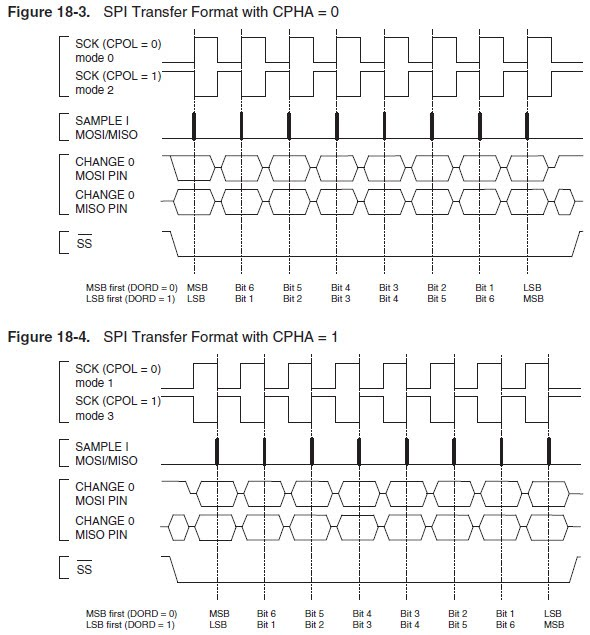
\includegraphics[scale=0.5]{fig11.jpg}
		\centering
		\caption {Modos de Operação de SPI}
		\label{fig:figura11}
	\end{figure}

\newpage

\subsection*{Comunicação Série Sincrona:I2C}

É usado para ligar periféricos mais lentos ao processador e admite mais que um master( Multi-Master).

Os dispositivos que estiverem ligados ao bus têm um endereço unico para cada um deles.O master representa qualquer dispositivo que tenha capacidade de iniciar mensagens no bus assim como é aqule que gera o relógio e inicia a comunicção com os slaves.Quanto ao nó slave este apenas recebe o clock e responde quando é endereçado pelo master. Neste protocolo o bus é multimaster pelo que tem de haver arbitragem no bus.

\subsubsection*{Comunicação no bus}

A comunicação entre dispositivos usualmente processa-se  seguindo a ordem:

\begin{enumerate}
	\item Espera até	que	não	haja	atividade no	bus	(SCL	e	SDA	ambos	high);
	\item Colocar uma mensagem no	bus	assinslando que	o	dispositivo assumiu o	controle do	bus	(tornou-se	master). Todos os outros	dispositivos ficam a	
aguardar ser endereçados;
  \item  Master	fornece o	sinal de	relógio na	linha	SCL.	Será	usado	por	todos	os	outros	 dispositivos	no	bus	como	a	indicação	do	intervalo	de tempo	em	que	cada	bit de	dados	na	linha	SDA	é	válido	e	pode	ser	usado.	O	dado	em	SDA 	tem	de	ser	válido	no	momento	das	transições	1->0	de	SCL;
 \item Master	coloca	em	SDA,	bit	a	bit,	o	endereço	do	dispositivo	com	que	quer comunicar Master	coloca	em	SDA	uma	mensagem	(1	bit)	indicando	se	pretende	enviar	(write)	ou	receber	(read)	um	dado	do	outro	dispositivo;
 \item  Master	verifica	se	o	outro	dispositivo	envia	um	bit	de	ACKNOWLEDGE	de	que	reconheceu	o	seu	endereço	e	está 	pronto	a	comunicar. 	\item Dados	podem	ser	transferidos;
\item O	master	envia	ou	recebe	tantos	bytes	quantos	quizer.	Depois	de	cada	byte	ser	enviado	o	dispositivo	que	o	enviou	espera	o	ACKNOWLEDGE	do	recetor;
\item Quando	todos	os	bytes	foram	enviados	o	master	liberta	o	bus	gerando	o	bit	de	STOP.
\end{enumerate}
\newpage
\subsubsection{Transferência de dados}

 	\begin{figure}[ht]
		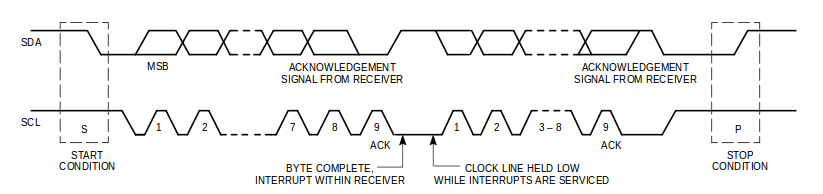
\includegraphics[scale=0.5]{fig12.png}
		\centering
		\caption {Transmissão de dados em I2C}
		\label{fig:figura11}
	\end{figure}

 	\begin{figure}[ht]
		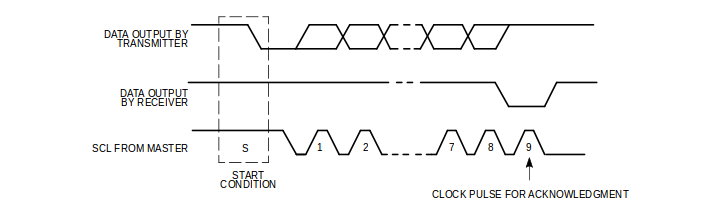
\includegraphics[scale=0.5] {fig13.png}
		\centering
		\caption {Aknowledge}
		\label{fig:figura11}
	\end{figure}

\subsubsection*{Sincronização do Relógio}

A sincronização de relógio surge com a existência de vários master sque podem, eventualmente, transmitir simultaneamente.A decisão de qual deles é que assume o contolo do bus pode ser feta usando este método.


\subsubsection*{Arbitragem}
A arbitragem processa-se bit a bit e, em cada bit quando SCL se encontra ativo cada master verifica se o valor de SDA coincide com o que enviou.Assim que um master envia um HIGH e verifica que o SDA está a LOW, este fica a saber que perdeu a prioridade e desliga o driver do bus.


\subsection*{Comunicação Série: CAN}

Controller Area Network é um bus de série multimaster com capacidade de tempo-real. Este bus foi concebido pela bus e é já o protocolo de referência automóvel e em medicina.

\subsubsection*{Caracterisitcas}
\begin{itemize}
 \item Bus Multi-Master assíncrono;
 \item Inexitência de enderessamento dos nós;
 \item Mecânismos avançados de deteção de erros;
 \item Taxa de bits até 10Mbit/s;
 \item Frequencias de Funcinamento que oscilam de 1MHz até 125 KHz;
 \item Comprimento Máximo:
 	\begin{itemize}
 	\item 1MHz -> 40m;
 	\item 125KHz -> 500m;
 	\item 50KHz -> 1Km; 
 	\end{itemize}
 \item è uma rede fechada, ou seja, é desnecessária a existência de segurnaça ou interface com o utilizador.
\end{itemize}

\subsubsection*{CAN higher Level Protocols}

Estes protocolos são usados para standardizar os procedimentos \textit{startup}, distribuir endereços e os tipos das mensagens entre os nós, determinar a estrutura das mensagens e por fim, dornecer rotinas de processamento de erros ao nível do sistema.

\subsubsection*{Protocolo de Transmissão(Message Ortiented)}

O protocolo de transmissão caracteriza-se por cada nó ser um recetor e um transmissor.Cada mensagem é transmitida a todos os dispositivos ligados ao bus.Todos os nós Lêem a mensagem e decidem se esta é relevante(filtering), e em cada nó há verificação de erros.A transmissão usa NRZ.

\subsubsection*{Acesso ao BUS-Ethernet CSMA/CD}

\begin{itemize}
	\item CS(Carrirer Sense)-> cada nó faz a monitorização do bus por forma a detectar periodos de inatividade antes de eniar as mensagens.
	\item MA(Multiple Access) -> Quando há um período de inatividade os nós têm a mesma priridade para enviar uma mesnsagem
	\item CD(Collision Detection) -> se 2 nós começam a transmitir em simultâneo os nós detetam a colisão e tomam medidas:
	\begin{itemize}
		\item Ethernet: os nós abortam a transmissão e tentam emitir outra vez após um delay.
		\item CAN: A situação acima descrita não pode ser aplicada no CAN pois é um protocolo de tempo real.Por isso a arbitragem é feita de modo a que a mensagem com maior prioridade seja transmitida sem corrupção e quaisquer atrasos.
	\end{itemize}
\end{itemize}

\newpage

\subsubsection*{CAN:CSMA/CA}

À semelhança do que foi descrito acima o Can não pode usar usar a deteção de colisão, ao invés disso atribui prioridades,usando identificadores, ás mensagens por forma a evitar colisões.
Quanto menor for o identificador  maior a prioridade.

 	\begin{figure}[ht]
		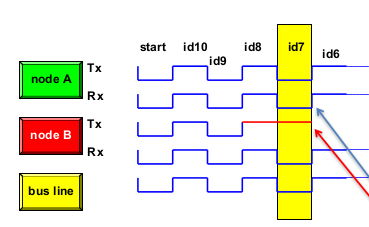
\includegraphics[scale=0.5] {fig14.png}
		\centering
		\caption {Método de transmissão de ID's}
		\label{fig:figura11}
	\end{figure}


\subsubsection*{Tipos de Mensagem}

\begin{itemize}
	\item Data Frame: usado quando um	nó transmite informação aos outros nós da rede;
	\item Remote Frame:basicamente uma data	frame	com	o	bit RTR	(Remote	Transmit Request) set	(=	1), significando que	se trata de	um	pedido de	transmissão remoto;
	\item Error Frame:geradas por nós que detetam um erro do protocolo;
	\item Overload Frame:geradas por nós que precisam de mais tempo para processar as mensagens recebidas;
	\item Interframe:as Data Frame e Remote Frame são separadas temporalmente por uma interframe;
\end{itemize}

	 	\begin{figure}[ht]
		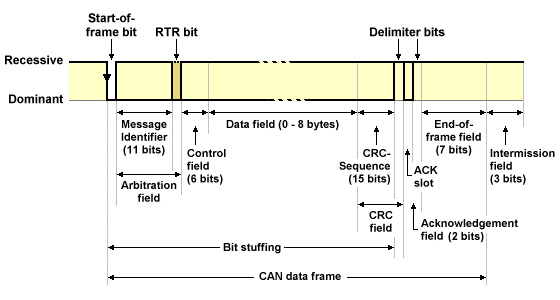
\includegraphics[scale=0.5] {fig15.png}
		\centering
		\caption {CAN Extended Data Frame}
		\label{fig:figura11}
	\end{figure}
	
	\begin{figure}[ht]
		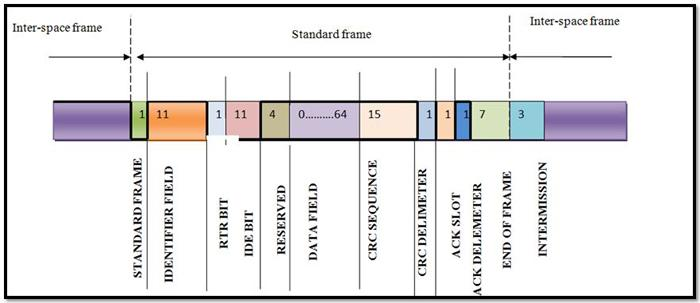
\includegraphics[scale=0.5] {fig16.JPG}
		\centering
		\caption {CAN Standard Data Frame}
		\label{fig:figura11}
	\end{figure}

\subsubsection*{Bit-Stuffing}
Quando se usa o código de NRZ caso não haja várias transições ao longo do tempo os relógios não vão conseguir sincronizar o seu relógio.Surge então o bit stuffing que casohajam cinco bits em que a informação faz com que seja inserido um bit com nivel lógico diferente por forma a resincronizar.


\subsubsection*{Erros em CAN}
\begin{itemize}
	\item Bit-Error: bit transmitido não é lido com o valor devido;
	\item Bit-Stuff-Error:Mais de 5 bits seguidos com o mesmo valor;
	\item CRC-ERROR: A soma CRC recebida não coincide com a calculada;
	\item Format Error: Violação do formato da mensagem;
	\item Aknowledgement Error: Ocorre quando otransmissor não recebe o dominant bit durante o aknowledgement slot.
\end{itemize}

\paragraph{CAN Error Handling  Sequence}

Quando é detectado um erro por um nó é transmitida uma error frame para todos os nós, de sequida a última mensagem recebida é eliminada em todosos nós, os contadores de erro são incrementados e por fim a mensagem é retransmitida.

Existem três estados de erro:
\begin{itemize}
	\item Error Active: modo normal de operaçã.Permite ao nó transmitir e receber mensagens sem restrições. Caso haja um erro é emitida uma Active Error Frame;
	\item Error Passive: após a deteção deu um determinado numero de erros é lançado este estado.Quando neste estado o nó pode receber e transmitir mensagens.
	\item Bus OFF: quando o contador de erros de transmissão excede o seu limite o nó é separado da rede CAN, não sendo permitidas quaisquer troca de mensagens.Não é transmitida uma error frame e só é possível recuperar deste estado fazendo um reset.
\end{itemize} 

	\begin{figure}[ht]
		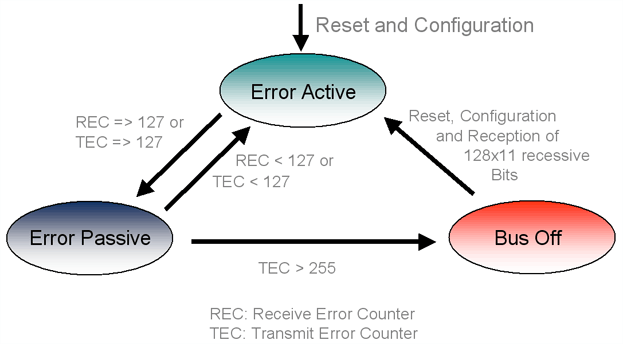
\includegraphics[scale=0.5] {fig17.png}
		\centering
		\caption {Diagrama Temporal do Contador de Erros}
		\label{fig:figura11}
	\end{figure}

\subsection*{USB}

O USB surgiu com o objectivo de facilitar a ligação de periféricos ao computador pessoal com uma única ficha e um unico protocolo.

É um bus single-master em que o host é o único componente master e todos os periféricos que se ligam ao  computador são slaves.

\subsubsection*{Transeferência de Dados}

As transferências de dados efectuam-se entre o software(device driver) e um endpoint  existente no dispositivo.

O Endpoint é um buffer onde dados entram e saem do USB são armazenados. Um in endpoint é um dispositivo que fornece dados ao host.Analogamente  um out endpoint recebe informações vindas do host.

Um conjunto de endpoints é designado por Interface.Cada interface está associada a uma função exclusiva do dispositivo.É necessário um device driver para cada interface.

O pipe é a ligação lógica entre um software driver no host e um endpoint.Todos os dispositivos têem um control pipe que usa o endpoint zero.

Para enviar ou receber dados o host inicia uma transferência, cada uma dessas transeferências consiste numa transição, que por sua vez, envolve 2 ou três pacotes:
\begin{enumerate}
\item Token Packet;
\item Data Packet e ou Handshake Packet.
\end{enumerate}

\paragraph*{Tipos de Transferências de Dados(I/O packet requests):}
\begin{itemize}
\item Control Transfers: usadas para configurar o dispositivo quando este é ligado;
\item Interrupt Data Transfers:o host interroga periódicamente o periférico.Usados para transmitir poucos dados num intervalo de tempo definido;
\item Bulk Data Transfers: transferência de uma grande quantidade de dados, mas sem grande importância temporal;
\item Isochronous Data Transfers: trnsferências em tempo real, ou seja com um baixo tempo de latência.
\end{itemize}

\paragraph*{Transferências de Controle}

Este tipo de transações ocorrem durante o processo de inicialização de comandos, estas suportam a comunicação de configuração , comandos e status entre o software do host e a função especifica comunicando com o endpoint 0 do dispositivo.
Iniciam-se sempre com uma fase de setup(configuração) e terminam com uma de status(estado)
As transferências de control são o mecanismo para aceder aos descrtores dos dispositivos e para formular pedidos ao dispositivo quanto ao seu funcionamento.

\subsubsection*{Frames}

É através do envio de frames que se processam as transferências no bus do USB.

Cada frame contem 1500 bytes.90\% da largura de banda do bus é utilizada para frames, a restante para Bulk Transfers e comandos.

\newpage

\section*{Memória}
A memória é um dos elementos mais importantes de um computador. É aí que são armazenados os dados e as instruções.Porém estas apresentam limitações a niveis fisicos.Por exemplo, uma maior velocidade de acesso implica não só maior consumo de energia como também é mais dispendioso por bit, outro problema é que quanto maior a capacidade da memória menor é a velocidade de acesso.


\subsection*{Hierarquia de Memória}


Surge então a necessidade de separar as memórias em vários tipos sendo cada um deles mais apropriado para uma determinada função.Podemos então dividir as memórias em três grupos essenciais estabelecendo uma hierarquia:
\begin{enumerate}
\item Cache;
\item Memória Central ou SDRAM;
\item Mémória de Massa
\end{enumerate}

Quanto maior onumero dessa hieráriquia maior vai ser a sua capacidade,porém a velocidade de acesso à mesma vai diminuir como pode ser observado na figura 18 .

	
	\begin{figure}[ht]
		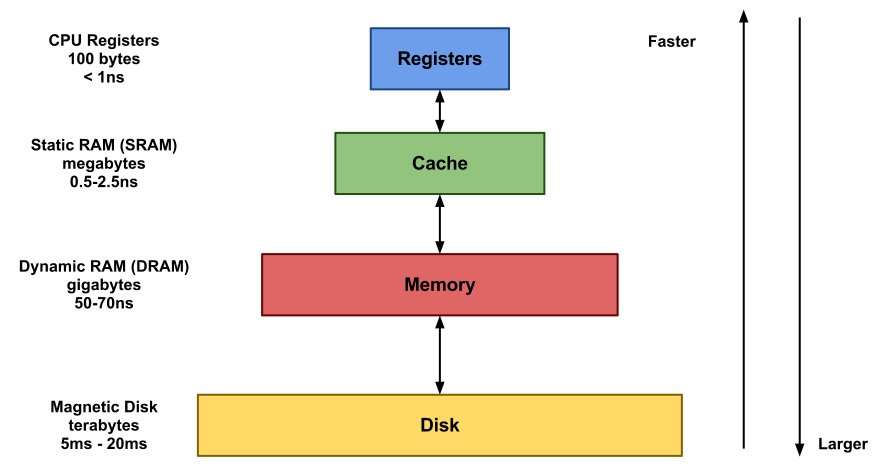
\includegraphics[scale=0.35] {fig18.png}
		\centering
		\caption {Hierárquia de Memória}
		\label{fig:figura18}
	\end{figure}


\subsubsection*{Funcionamento da Hierarquia de Memória}

Existem dois critérios que permitem saber em que memórias se devem armazenar os dados.
A localidade temporal afirma que se devem manter os dados que sao acedidos mais vezes na memória mais rápida e por sua vez a localidade espacial afirma que os blocos vizinhos devem ser movidos para a memória mais rápida.

Um dos grandes ganhos deste método é garantir ao utilizador a maior capacdade e velocidade com a tecnologia mais barata.





\end{document} 